\subsection{Network Offloading Performance}
\label{subsec:network-offloading-eval}
%\paragraph{Latency metric}
We evaluate a full-body DAG configuration in which motion processing imposes substantial computational load. 
Two execution modes are compared: (1) client-only processing, where all nodes execute locally, and (2) server offloading, where selected computational nodes are migrated to the server while tracking remains client-driven. 
Under the offloading configuration, downstream motion processing and avatar transformations are executed server-side.

We evaluate network offloading performance by measuring application-level input-to-photon (ITP) latency as a proxy for interaction latency.
Total latency comprises client processing time, network upload, server processing time, and network download between frames.
Reported measurements reflect the tested client–server topology and network conditions and may vary under different node compositions. 
Sensor sampling, runtime compositor latency, and display scan-out are excluded from this analysis. 
To ensure stable statistics, we discard the initial 10\,s as a warm-up period and restrict analysis to samples with latency \(\leq 200\)\,ms.

\begin{table}[t]
\centering
\caption{Server and client hardware specifications used in offloading performance experiments.}
\label{tab:hardware-spec}
\begin{threeparttable}
\scriptsize
\begin{tabular*}{\columnwidth}{@{\extracolsep{\fill}}lccc@{}}
\toprule
   & PC & Meta Quest 3 & XREAL X4000 \\
\midrule
CPU             & Xeon 6246R & SD$^\dagger$ XR2 Gen2 & SD$^\dagger$ 8 Gen1 \\
Clock (GHz)     & 3.40   & 2.05             & 1.80 \\
Processors      & 2          & 1                    & 1 \\
Cores/Threads       & 32/64         & 8/8                    & 8/8 \\
\bottomrule
\multicolumn{4}{@{}p{\columnwidth}@{}}{$^\dagger$ SD stands for Snapdragon}
\end{tabular*}
\end{threeparttable}
\end{table}

% Added short narrative for the hardware table
{\bf Table~\ref{tab:hardware-spec}} summarizes the test platforms. 
The server system is a dual-socket Intel Xeon 6246R (3.40\,GHz; 32 cores, 64 threads). 
The Meta Quest~3 client integrates a Snapdragon XR2 Gen~2 SoC (8 cores at 2.05\,GHz), while the XREAL X4000 uses a Snapdragon 8 Gen~1 SoC (8 cores at 1.80\,GHz). 
Both HMDs are single-processor devices without exposed SMT. 



\begin{table}[t]
\caption{ITP latency summary statistics (mean$\pm$SD, p50, p95, p99, range) for client-only and offloaded execution.}
\label{tab:network-analysis} 
\centering
\setlength{\tabcolsep}{0.75\tabcolsep}
\renewcommand{\arraystretch}{1.5}
\scriptsize
\begin{tabular*}{\columnwidth}{@{} p{29pt} p{29pt} ccccc @{}}
\toprule
Hardware & Comm. Config. & Mean & p50 & p95 & p99 & Range \\
\midrule
Meta Quest 3
  & Self-feed & 15.3 $\pm$ 2.6 & 15.0 & 18.9 & 27.0 & 6.7--33.6 \\
  & Offload & 13.9 $\pm$ 0.4 & 13.9 & 14.5 & 14.9 & 8.7--18.4 \\
\midrule
XREAL X4000
  & Self-feed & 28.3 $\pm$ 8.9 & 30.4 & 39.7 & 48.3 & 9.5--76.0 \\
  & Offload & 20.3 $\pm$ 7.3 & 18.7 & 33.3 & 36.1 & 5.6--42.2 \\
\bottomrule
\end{tabular*}
\end{table}


\begin{figure}[t]
  \centering

  % ---------- Row 1: center the pair as a group ----------
%   \makebox[\linewidth][c]{%
    \begin{subfigure}[t]{0.49\linewidth}
    \centering
    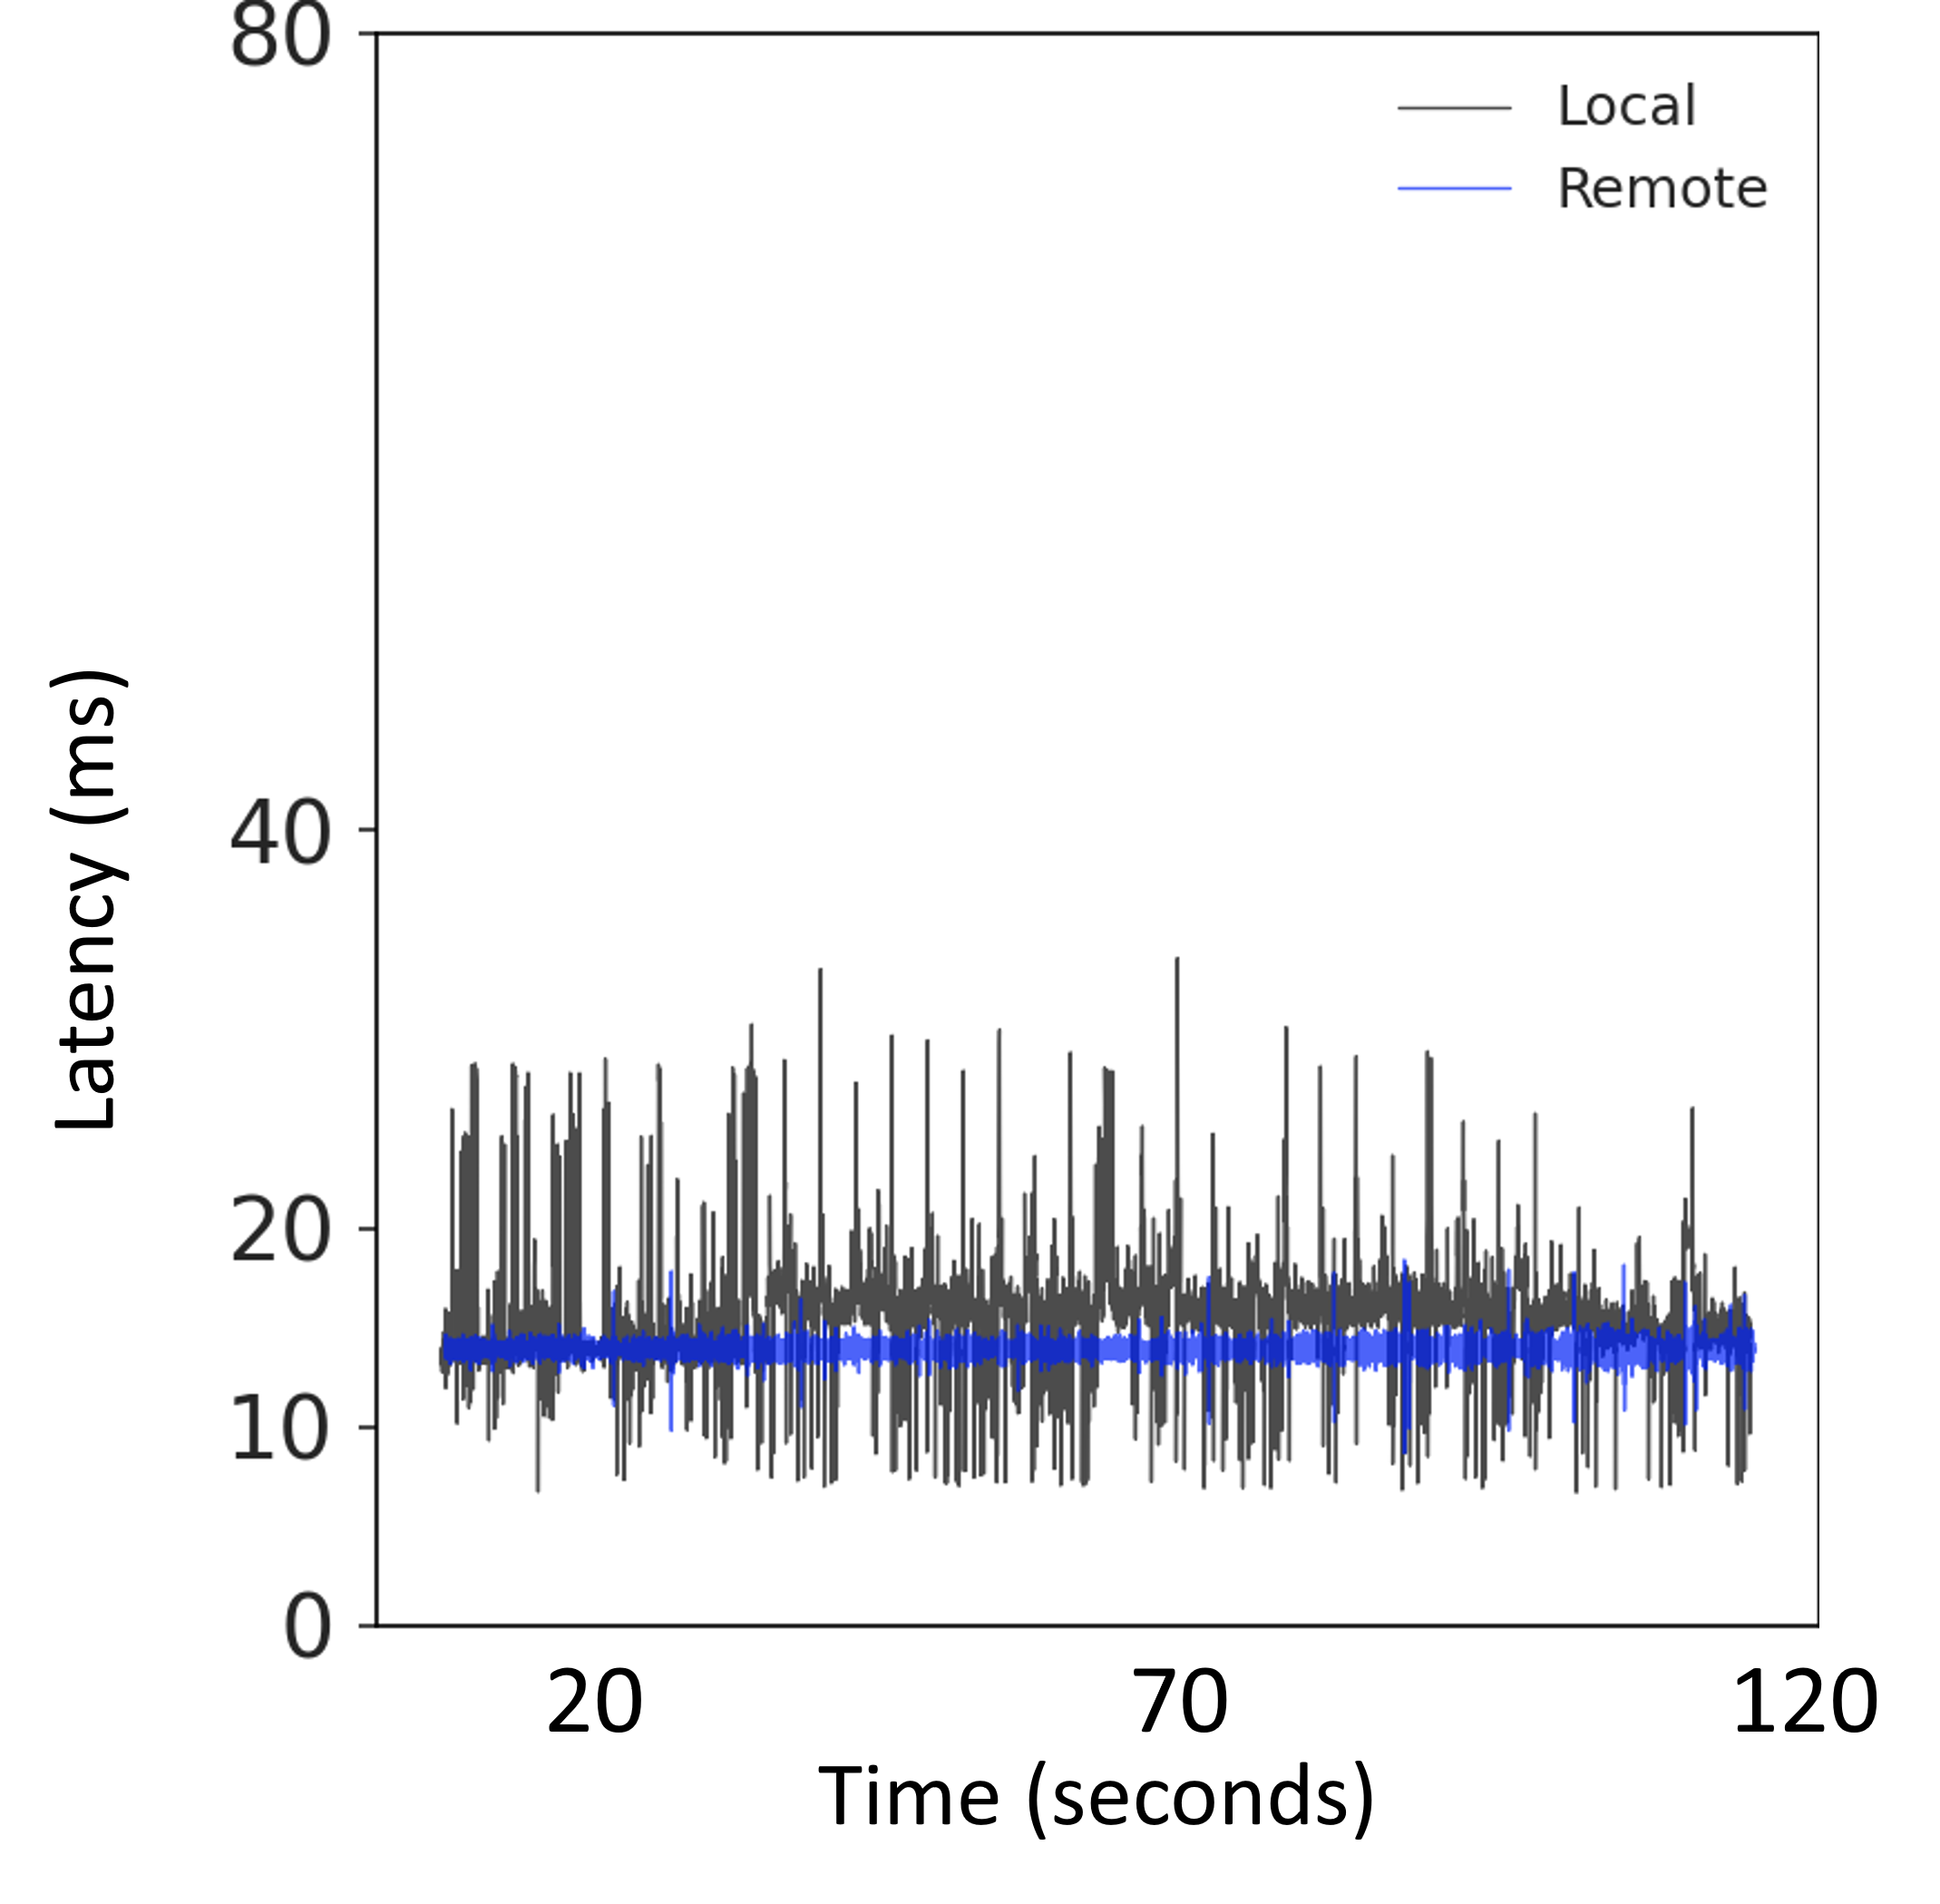
\includegraphics[height=3.75cm,keepaspectratio]{figures/latency/figures/latency_quest3.png}
    \subcaption{Latency in Quest3}
    \label{fig:network-analysis:a}
    \end{subfigure}\hfill
    \begin{subfigure}[t]{0.49\linewidth}
    \centering
    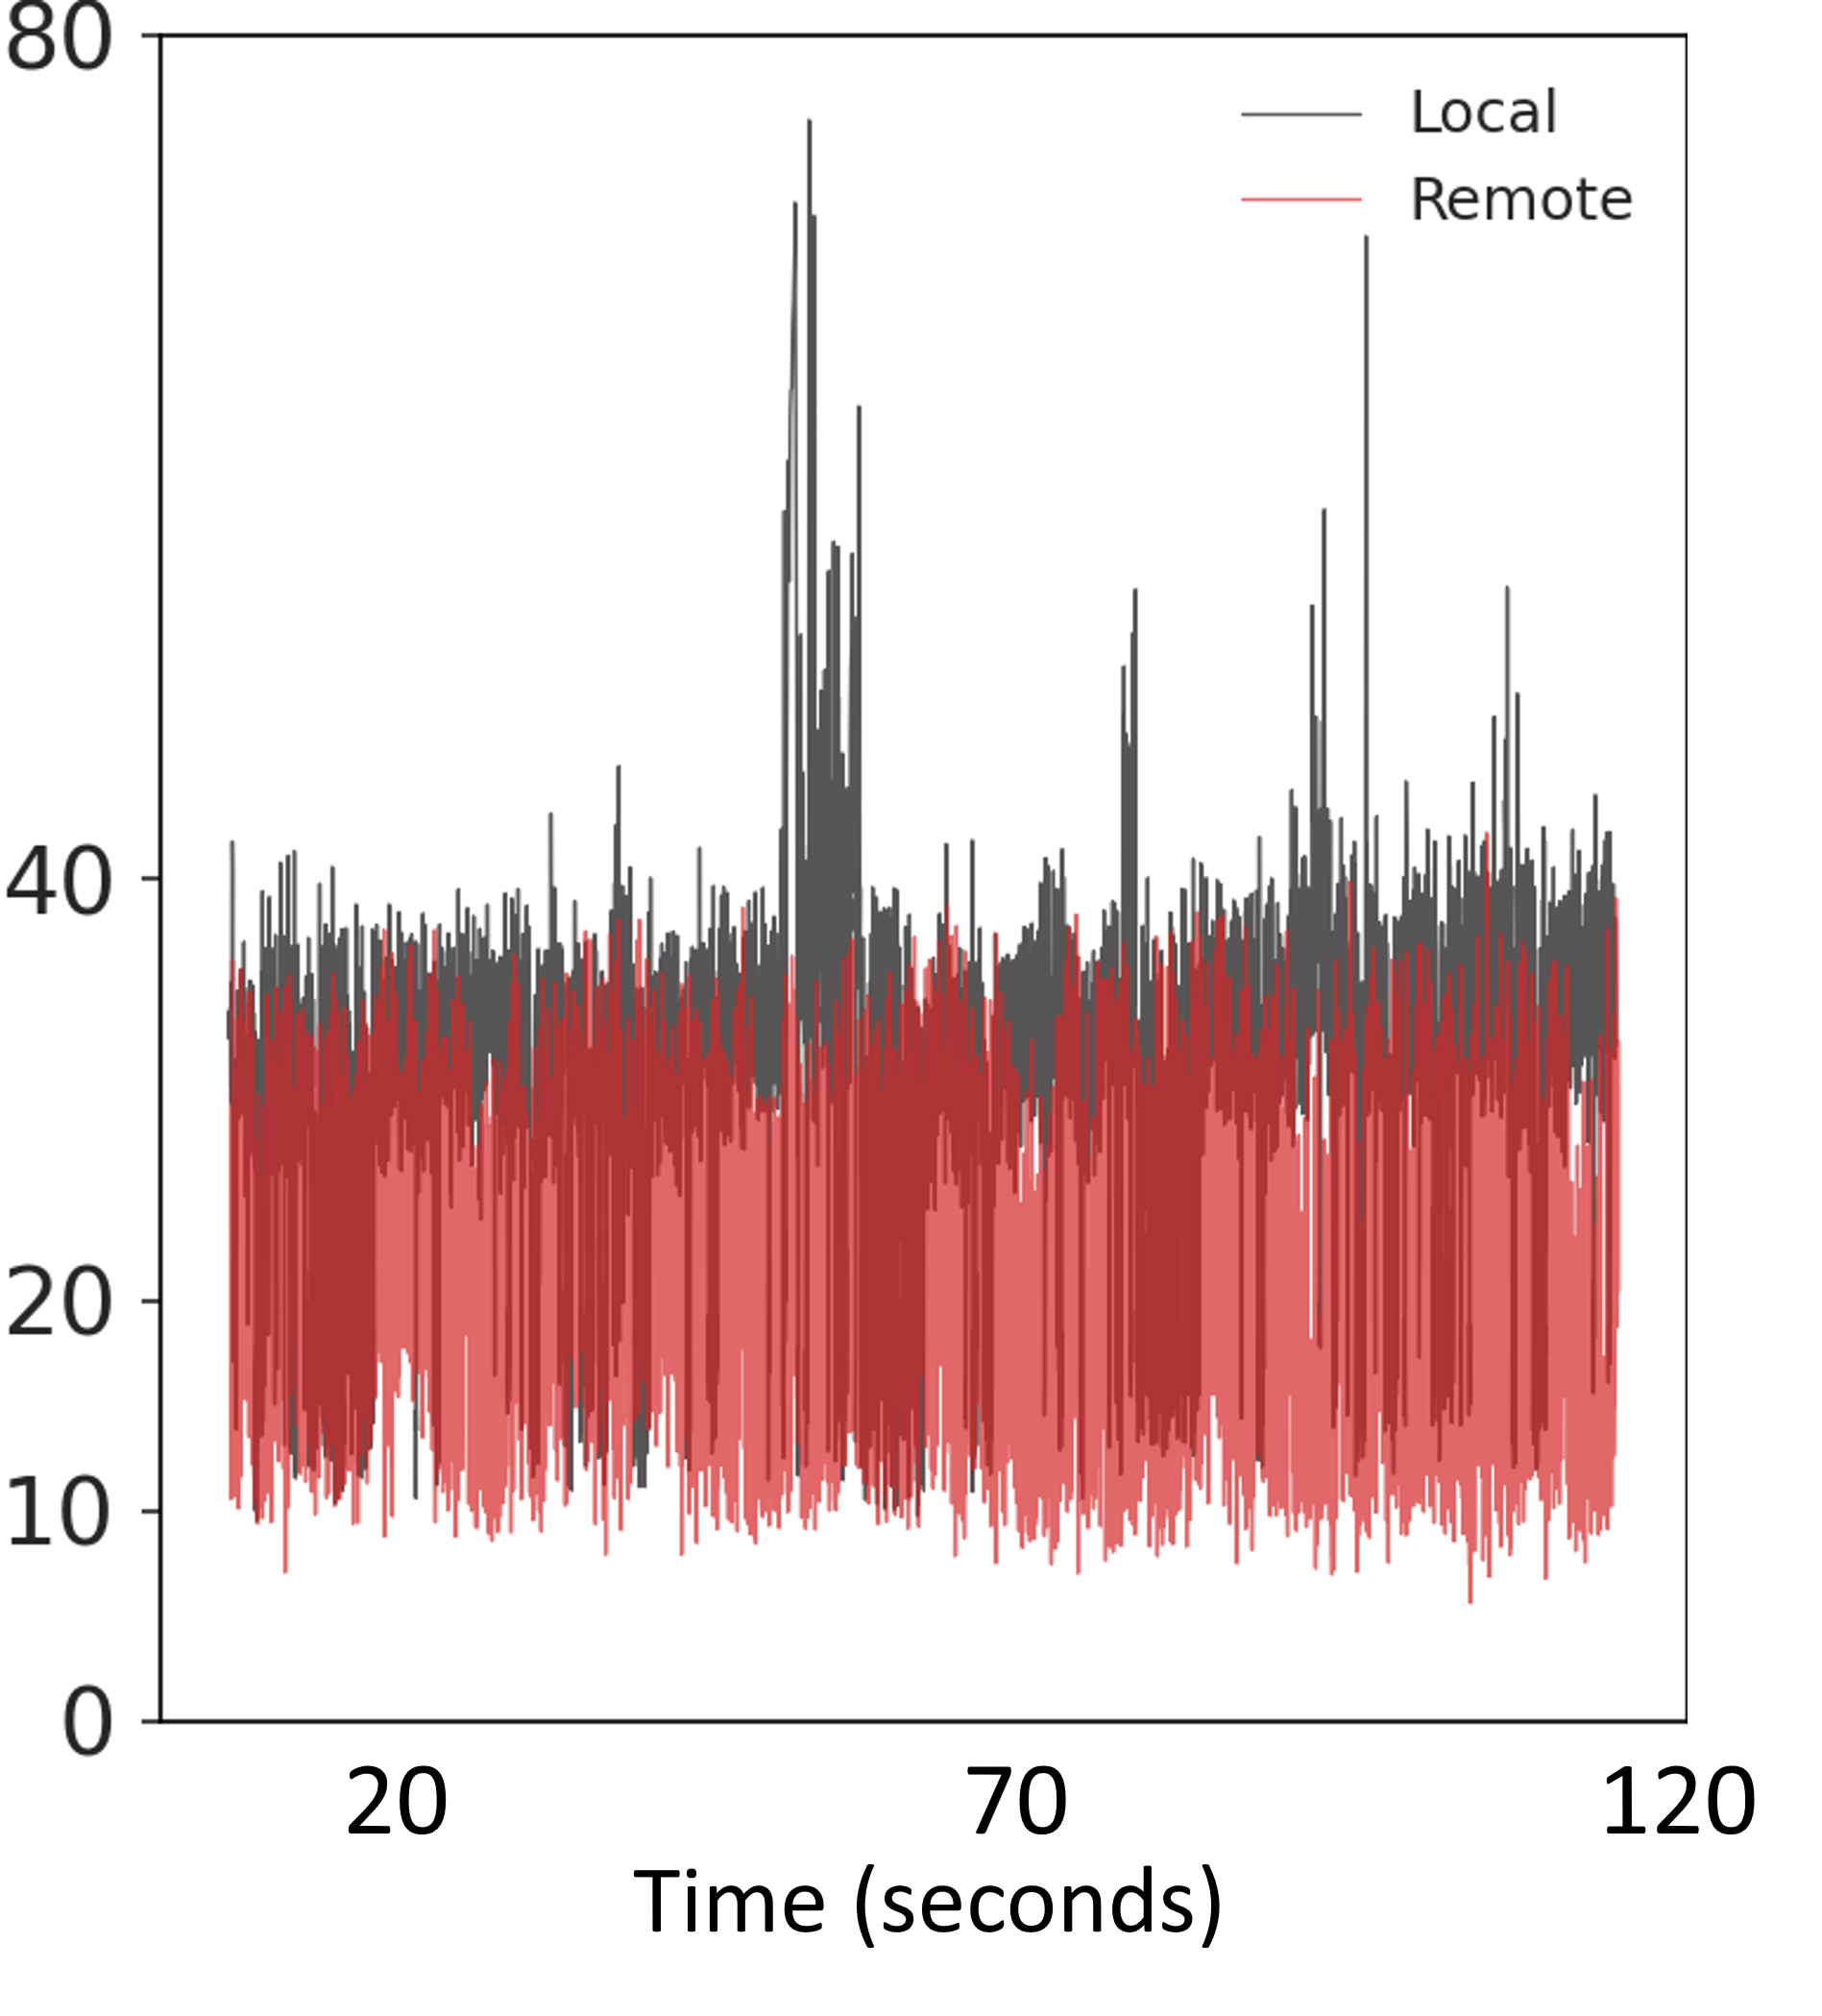
\includegraphics[height=3.75cm,keepaspectratio]{figures/latency/figures/latency_xreal.png}
    \subcaption{Latency in XREAL}
    \label{fig:network-analysis:b}
    \end{subfigure}
%   }

  \vspace{0.5em} % vertical gap between rows

  % ---------- Row 2: same idea ----------
  \makebox[\linewidth][c]{%
    \begin{subfigure}[t]{0.49\linewidth}
      \raggedleft
      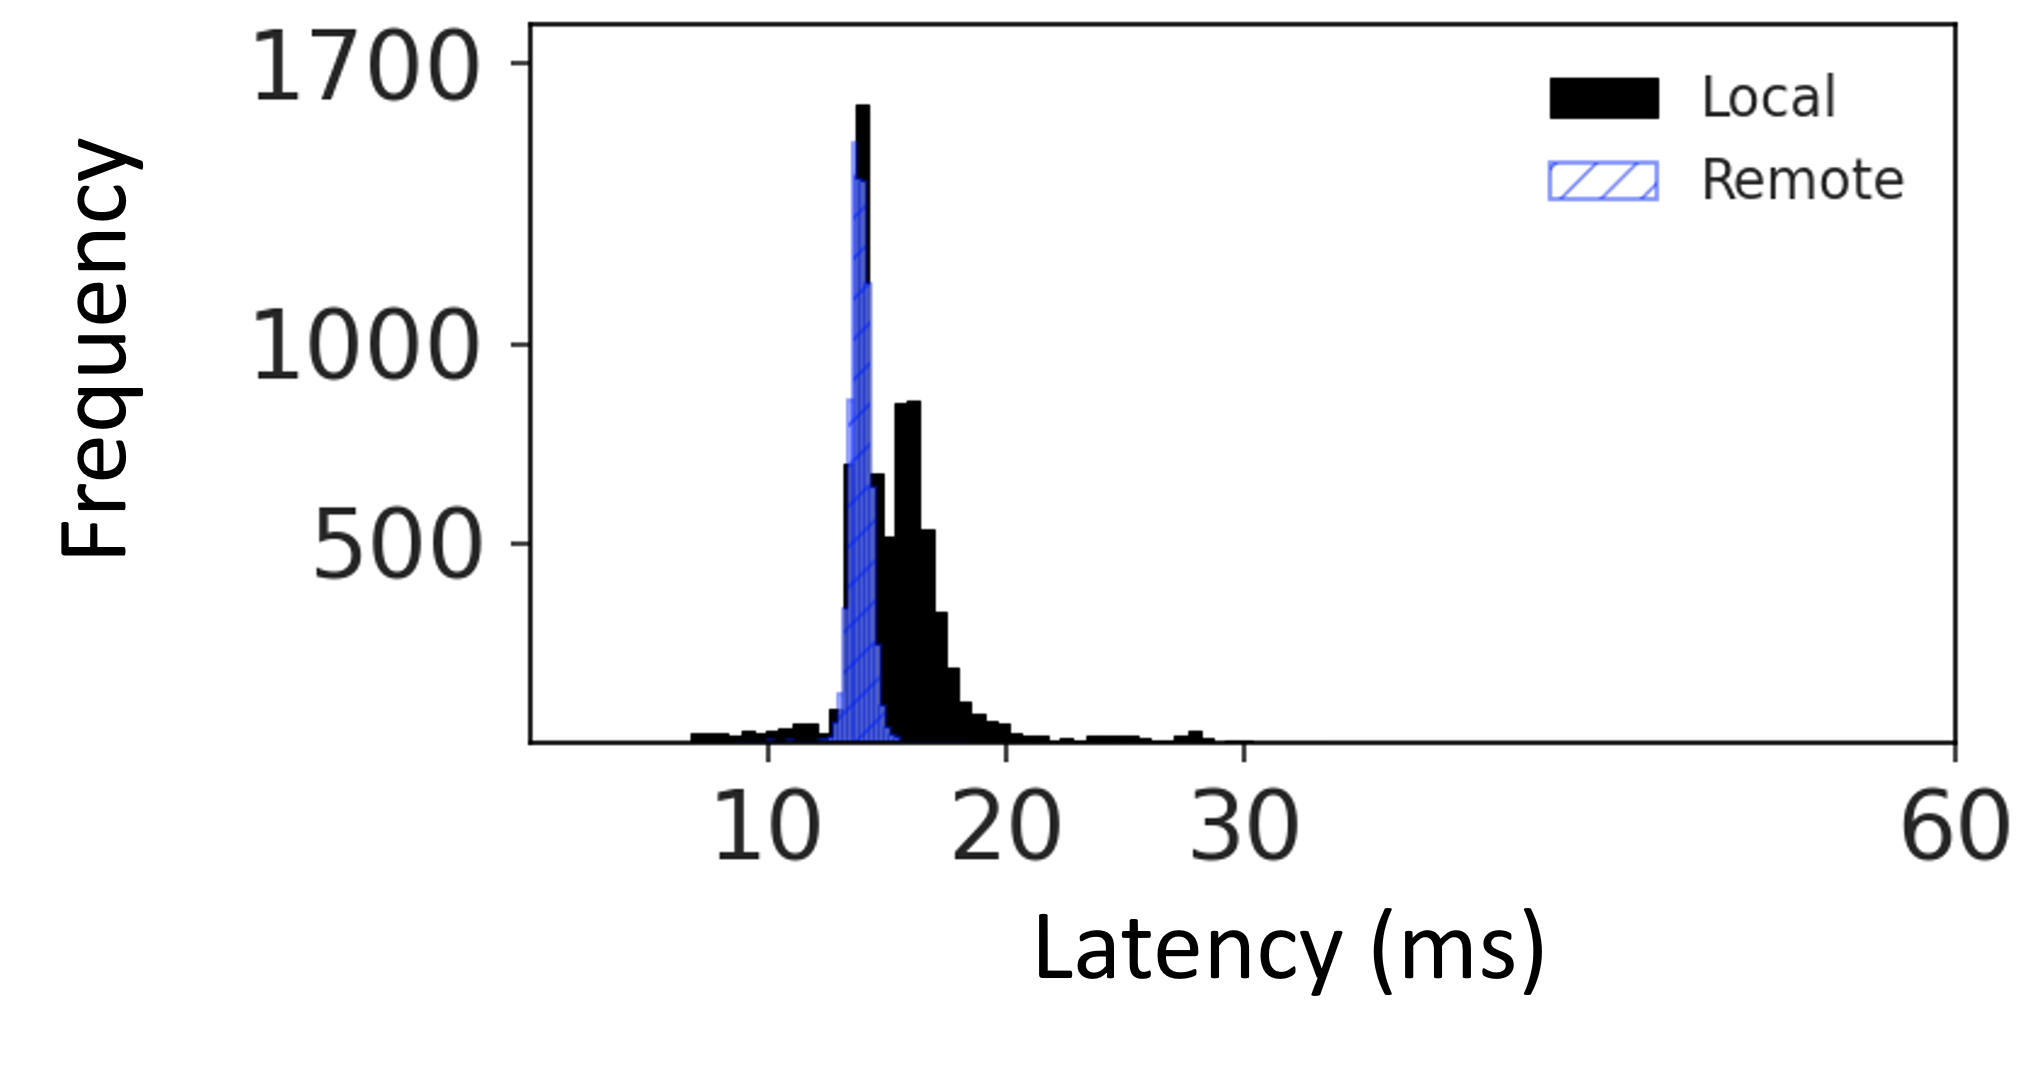
\includegraphics[height=2.1cm,keepaspectratio]{figures/latency/figures/frequency_quest3.png}
      \subcaption{Latency dist. in Quest3}
      \label{fig:network-analysis:c}
    \end{subfigure}\hfill
    \begin{subfigure}[t]{0.49\linewidth}
      \raggedright
      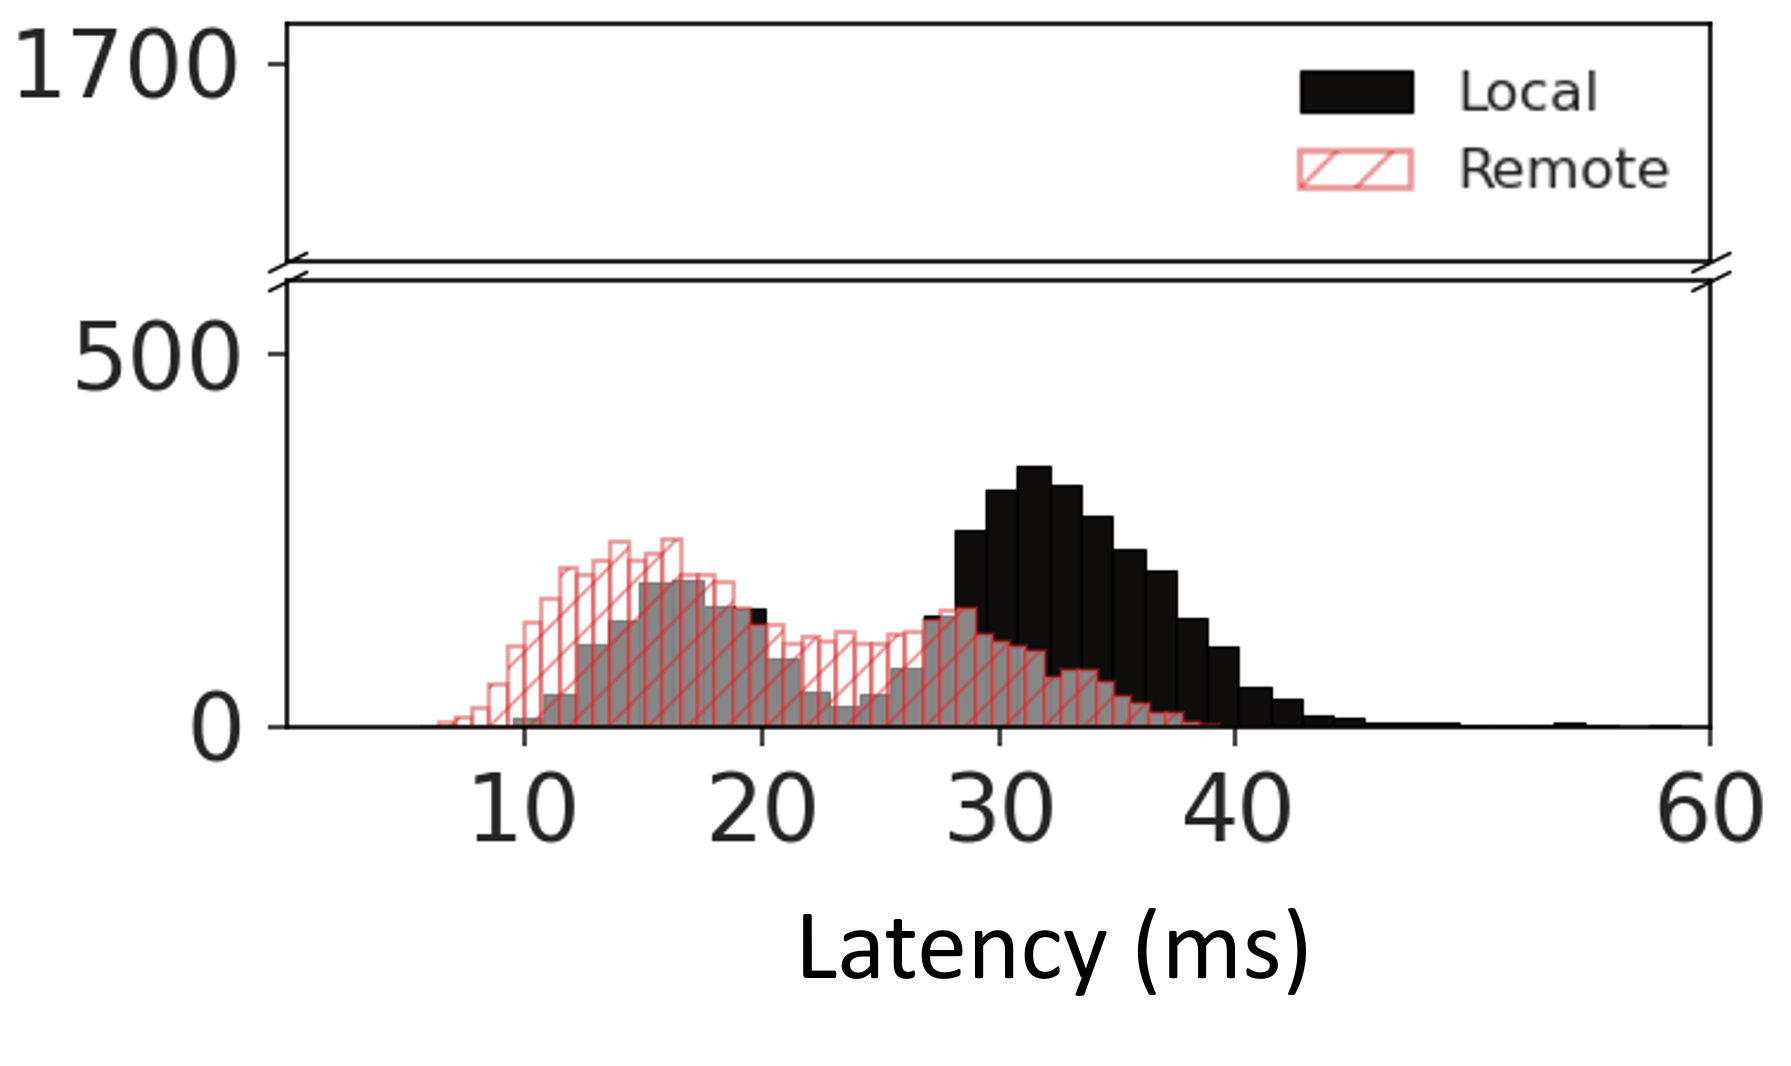
\includegraphics[height=2.1cm,keepaspectratio]{figures/latency/figures/frequency_xreal.png}
      \subcaption{Latency dist. in XREAL}
      \label{fig:network-analysis:d}
    \end{subfigure}%
  }

  \caption{Interaction latency and distribution for local vs offloaded on Quest 3 and XREAL X4000.}
  \label{fig:network-analysis}
\end{figure}

{\bf Figure~\ref{fig:network-analysis}} presents latency time-series and corresponding distributions for client-only and offloaded configurations on Quest~3 and XREAL X4000. Interaction latency is defined as the interval between a 6DoF input event and the subsequent visual update on the HMD. 

Quest~3 under client-only execution exhibited a median of 15.0\,ms (mean 15.3$\pm$2.6\,ms) with a long tail up to p99 $=27.0$\,ms and a range of 6.7--33.6 ms. With server offloading, the distribution shifted left (p50 $=13.9$\,ms; mean 13.9$\pm$0.4\,ms), and tail latency contracted substantially (p95: 18.9$\rightarrow$14.5\,ms; p99: 27.0$\rightarrow$14.9\,ms). 
Time-series traces indicate reduced jitter and fewer transient spikes under offloading.

On XREAL X4000, client-only execution showed higher and more variable latency (median 30.4\,ms; mean 28.3$\pm$8.9\,ms; p95 $=$39.7 ms, p99 $=48.3$\,ms). 
Offloading shifted the distribution toward lower latency (p50 $=18.7$\,ms; mean 20.3$\pm$7.3\,ms) and reduced tail behavior (p95: 39.7$\rightarrow$33.3\,ms; p99: 48.3$\rightarrow$36.1\,ms). The time-series similarly shows fewer high-latency excursions despite added network round-trip and encoding overhead.

Across both devices, server offloading reduced central tendency and tail ITP latency, with larger absolute gains observed on XREAL X4000.
On Meta Quest~3, client-only execution already achieves p95$<20$\,ms; offloading primarily reduces tail latency, which improves frame-to-frame consistency and reduces perceptible hitches during fast interactions. 
On XREAL X4000, offloading shifts the central tendency in addition to reducing tail latency, suggesting improved responsiveness for interaction-intensive tasks such as near-field manipulation and ray-based selection.

These findings have implications for XR system design: percentile-based targets, rather than means, should guide interaction-loop budgeting.
Under conditions similar to our experiments, Meta Quest~3 with offloading supports a conservative upper bound near p99$=14.9$\,ms, whereas XREAL X4000 with offloading supports p95$=33.3$\,ms for mid-complexity tasks. 
Buffering, late-latching, and prediction strategies should therefore be calibrated to the observed latency distributions--shorter fixed buffers suffice on Meta Quest~3, while slightly larger buffers and more aggressive prefetching may be appropriate on XREAL X4000. 
Finally, an on-device fallback path can help prevent p99 degradation under network impairment. All measurements were obtained under the specific network and workload conditions described above; practical deployment should re-estimate p50, p95, p99, and range in situ.


% XREAL None
% 108.3 ~ 150.0ms
% 112.5 ~ 166.7
% 125.5 ~ 191.2
% offload
% 62.5 ~ 
% 66.7 ~ 104.2
% 70.8 ~ 116.7
% 75.5 ~ 125.0
% 79.2 ~ 133.3
% 91.7 ~ 183.3

% Meta pro None
% 50.0 ~ 79.2
% 54.2 ~ 91.7
% offload
% 45.8 ~ 70.8
% 54.2 ~ 83.3
